\documentclass[a4paper,12pt]{article}	% тип документа

\usepackage[a4paper,top=1.3cm,bottom=2cm,left=1.5cm,right=1.5cm,marginparwidth=0.75cm]{geometry} % настройка полей

\usepackage[T2A]{fontenc}			% кодировка
\usepackage[utf8]{inputenc}			% кодировка исходного текста
\usepackage[english,russian]{babel}	% локализация и переносы
\usepackage{indentfirst}

%Рисунки
\usepackage{graphicx}

\usepackage{wrapfig}

\usepackage{multirow}

\usepackage{float}

%Графики
\usepackage{pgfplots}
\pgfplotsset{compat=1.9}

\usepackage[T1]{fontenc}
\usepackage{titlesec}

\setlength{\parindent}{3ex}

% Литература
\addto\captionsrussian{\def\refname{Литература}}

%Добавляет возможность искать и копировать текст
\usepackage{cmap}

%Убирает пробел между названием таблицы/рисунка и самой таблицей/рисунком
\usepackage{caption}
\captionsetup[table]{skip= -0 cm}
\captionsetup[figure]{skip= -0 cm}

%Выравнивание названия таблиц по левому краю
%\usepackage[nooneline]{caption}

%Рисунки
\usepackage{wrapfig} %обтекание элементов
\graphicspath{{graphs}{figures}} % папки с картинками

%Русский язык в формулах
%\usepackage{mathtext}

% Русский язык
\usepackage[T2A]{fontenc}
\usepackage[utf8]{inputenc}
\usepackage[english,russian]{babel}

%Готические буквы
\usepackage{amssymb}

% Математика
\usepackage{amsmath,amsfonts,amssymb,amsthm,mathtools}
\usepackage{wasysym}

% \cfoot{Нижний в центре} % По умолчанию здесь номер страницы

\begin{document} % the beginning of the document

% Title
\begin{titlepage}
	\begin{center}
		\large МИНИСТЕРСТВО ОБРАЗОВАНИЯ И НАУКИ РОССИЙСКОЙ ФЕДЕРАЦИИ\\
		МОСКОВСКИЙ ФИЗИКО-ТЕХНИЧЕСКИЙ ИНСТИТУТ \\
		(НАЦИОНАЛЬНЫЙ ИССЛЕДОВАТЕЛЬСКИЙ ИНСТИТУТ)\\
		ФИЗТЕХ-ШКОЛА ЭЛЕКТРОНИКИ, ФОТОНИКИ \\
		И МОЛЕКУЛЯРНОЙ ФИЗИКИ \\

	\vspace{4.0 cm}
	{Кафедра вакуумной электроники} \\
	\LARGE {Отчет по лабораторной работе} \\
	\LARGE \textbf{Растровый электронный микроскоп} \\
	\end{center}
	\vspace{3 cm} \large

	\begin{flushleft}
		\LARGE \textbf{Работу выполнили:} \hspace{0.8cm}  Коробкина Екатерина, Б04-107 \\
		
		\hspace{7.8cm} Марков Константин, Б04-105 \\
		
            \hspace{7.8cm} Нечаева Дарья, Б04-105 \\
            
            \hspace{7.8cm} Салтыкова Дарья, Б04-105 \\
           
            \hspace{7.8cm} Сифат Хасиб, Б04-105 \\
            
            \hspace{7.8cm} Шмаков Владимир, Б04-105 \\
		
	\end{flushleft}

	\vfill

	\begin{center}
		Долгопрудный, 2023 г.
	\end{center}
\end{titlepage}


	\newpage

\section{Введение}
	
\noindent \textbf{Цели}:

        \begin{itemize}
            \item изучение физических принципов работы РЭМ;

            \item изчение физических принципов формирования изображений в РЭМ;
            
            \item получение изображений образцов в различных режимах работы растрового электронного микроскопа (РЭМ).
            
        \end{itemize}

\noindent \textbf{В работе используются}: РЭМ JOEL JSM-7001F; образцы для электронно-зондового микроанализа (крыло бабочки, чипы).

\section{Теоретические сведения}

    \subsection{Вторичная электронная эмиссия}

\noindent Вторичная электронная эмиссия -- испускание электронов из твёрдого тела при бомбардировке пуском первичных электронов. Это явление представляет собой сложное наложение нескольких взаимосвязанных процессов: упругого и неупругого рассеяния первичных электронов, возбуждения внутренних, истинно вторичных электроно, их движения к поверхности и выхода в вакуум.

\medskip

\noindent Сложный характер явления вторичной электронной эмиссии наглядно проявляется в энергетическом спектре $N(E)$ вторичных электронов (рис. \ref{эл}).

    \begin{figure}[!h]
    	\centering{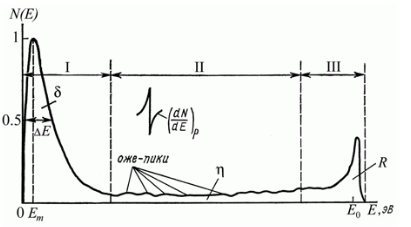
\includegraphics[scale=1]{2023-10-06_11-51.png}}
    	\caption{Энергетический спектр вторичных электронов.}
    	\label{эл}
    \end{figure}

    \begin{itemize}
        \item Область \MakeUppercase{\romannumeral 1} -- медленные истинно вторичные электроны ($0<E<50\ \text{эВ}$);
        \item Область \MakeUppercase{\romannumeral 2} -- неупругоотражёные первичные электроны ($50<E<2000\ \text{эВ}$);
        \item Область \MakeUppercase{\romannumeral 3} -- упругоотражённые первичные электроны.
    \end{itemize}

    Небольшие пики в областях \MakeUppercase{\romannumeral 1} и \MakeUppercase{\romannumeral 2} обусловленны оже-электронами.
    
    \subsection{Контраст в растровом электронном микроскопе}
    
\noindent Коэффициент вторичной электронной эмиссии зависит не только от элементного состава, но и от угла падения пучка, т.е. от рельефа поверхности. Так как глубина проникновения в вещество первичных электронов с энергией 20 кэВ составляет примерно $\sim$1 мкм (рис. \ref{ВЭ угол}). Однако вторичные электроны выходят из глубины примерно $30-50$ {\AA}  для металлов и $300-500$ {\AA} для диэлектриков. Поэтому, если превичный пучок электронов падает на образец под углом $\theta$, то при неизменной глубине выхода вторичных электронов размер области на поверзности образца, из которой они смогут выходить, увеличится как $\frac{Z}{\cos \theta}$, следовательно, увеличится и число вторичных электронов.

\medskip

\noindent По этой причине области на поверхности образца, на которые сканирующий пучок будет попадать под острыми углами, будут на изображении в РЭМ выгляжеть более светлыми. Кроме того, очень яркими будут выглядеть на изображении объекты с характерными размерами порядка глубины выхода электронов (пиролитические усы, нанотрубки и т.д.).

    \begin{figure}
    	\centering{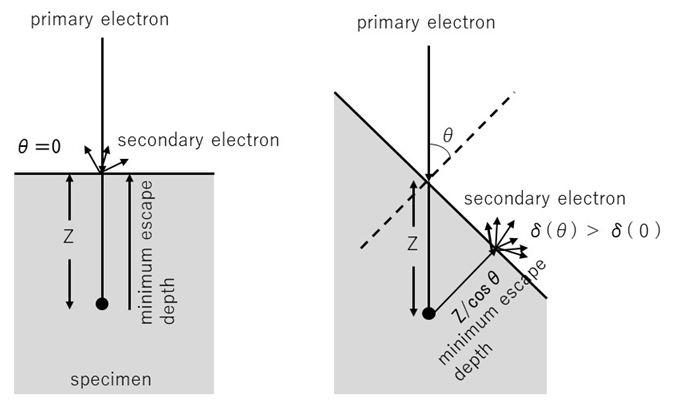
\includegraphics[scale=0.6]{кэ угол.jpg}}
    	\caption{Энергетический спектр вторичных электронов.}
    	\label{ВЭ угол}
    \end{figure}
    
    
\section{Общее устройство РЭМ}

    \begin{figure}[!h]
    	\centering{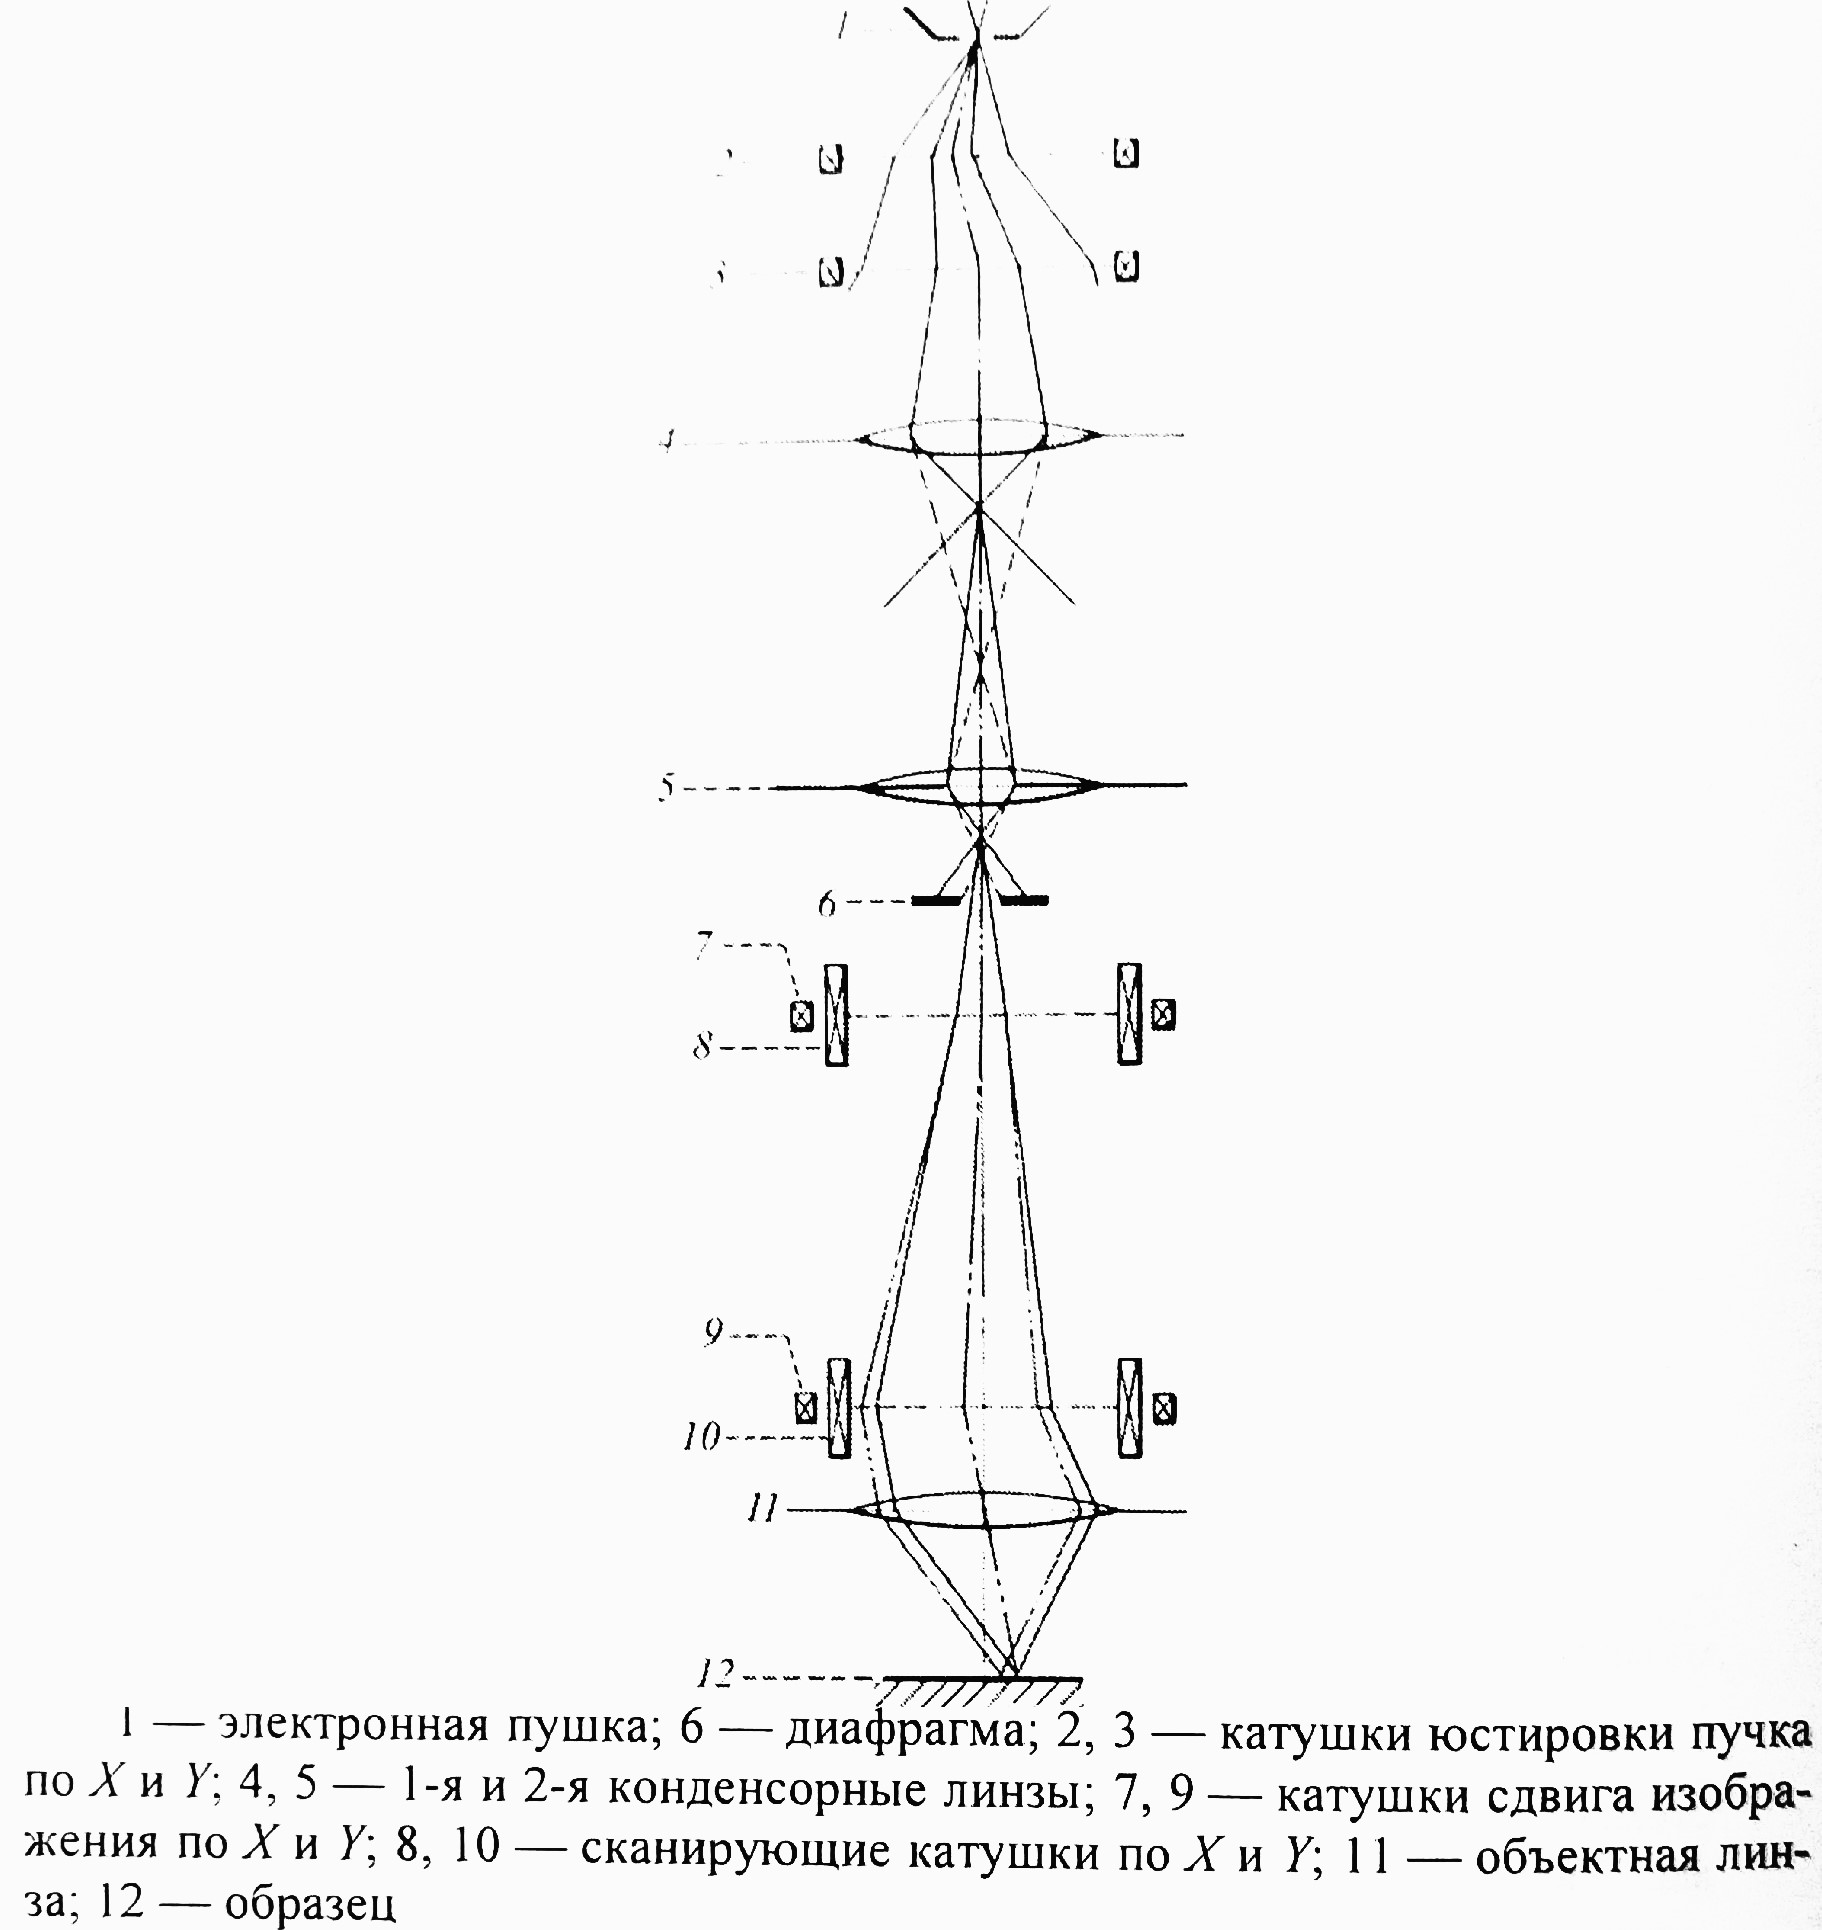
\includegraphics[scale=0.25]{SEM.jpg}}
    	\caption{Электронно-оптическая система.}
    	\label{ЭО сис}
    \end{figure}
    
\noindent Схема трехлинзовой электронно-оптической системы РЭМ JOEL JSM-7001F представлена на рис. \ref{ЭО сис}.

    \subsection{Электронный зонд}

\noindent В приборе используется вольфрамовый термополевой катод, испускающий электроны, которые проходят через цилиндр Венельта, на который подается еще более низкий потенциал. Цилиндр Венельта управляет током пушки, подобно сетке в электронной лампе. Будучи включённым в одну электрическую цепь с катодом, он позволяет нивелировать нестабильность потока электронов от вольфрамовой нити, которая зависит от температуры. С ростом температуры нити, возрастает и эмиссия электронов, но она достигает насыщения при определённой температуре. Напряжением между катодом и цилиндром Венельта можно регулировать уровень тока насыщения. Далее, электроны ускоряются на участке от цилиндра Венельта до анода, где происходит ускорение. Катод, цилиндр Венельта и анод образуют трехэлектродную пушку (см. рис. \ref{ЭО сис}), формирующей кроссовер в пространстве между цилиндром Венельта и анодом, диаметр которого зависит от фокусного расстояния пушки, анодного напряжения и температуры катода.

\medskip
        
\noindent Пройдя через отверстие в анодной пластине, электроны попадают в систему электромагнитных линз, при помощи которых формируется узкий зонд. Линзы представляют собой соленоиды, соосные электронному пучку. Они представляют собой цилиндрически симметричный электромагнит с очень острыми кольцевыми наконечниками полюсов, создающий в малой области сильное неоднородное магнитное поле, фокусирующее электроны, летящие вертикально через эту область.   

        \begin{figure}[h!]
            \centering{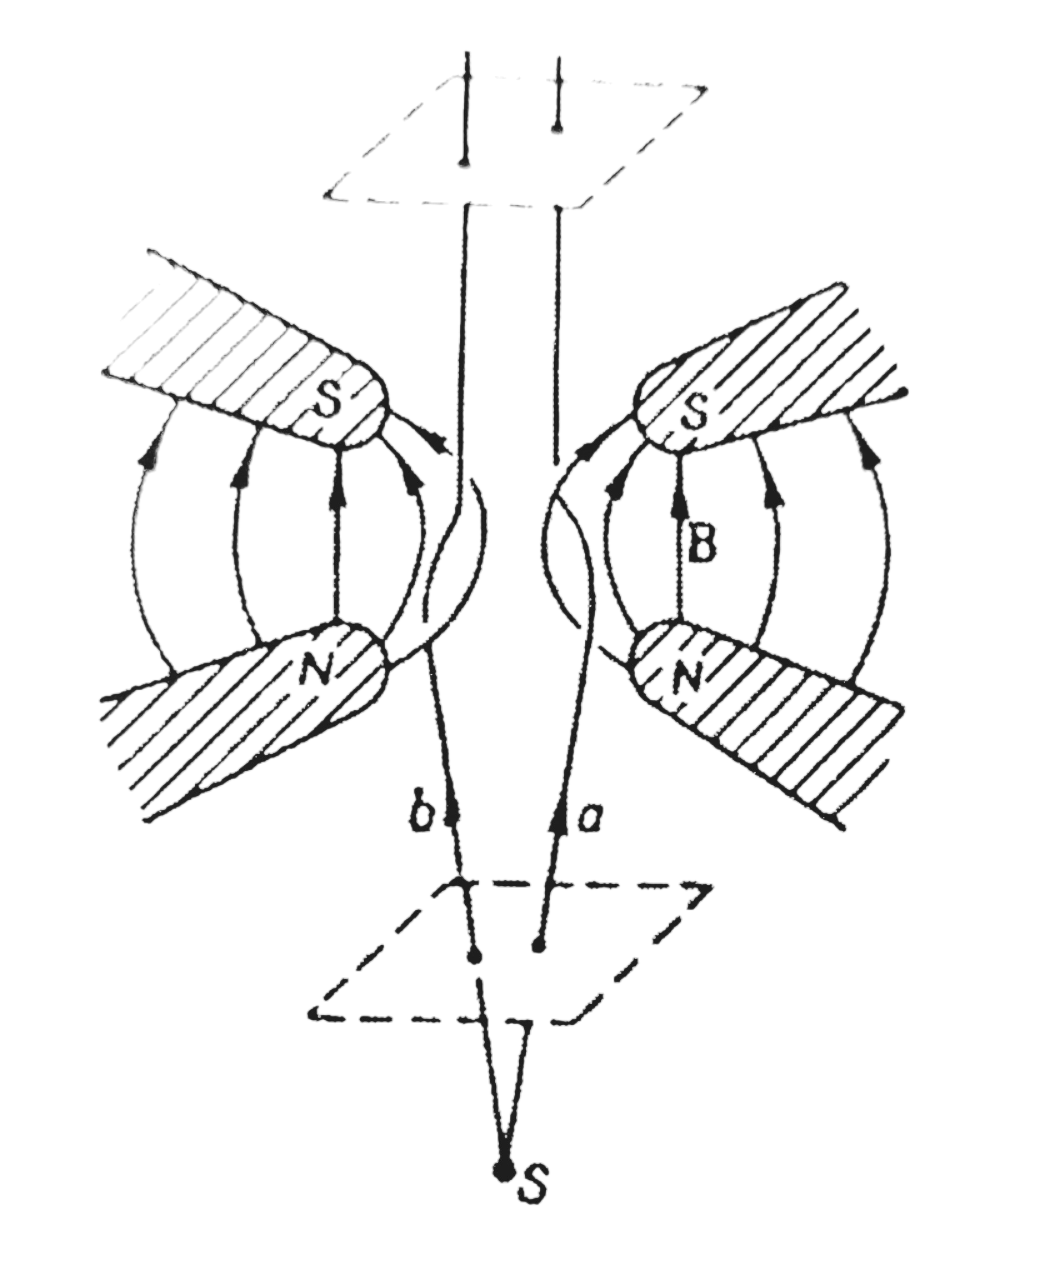
\includegraphics[scale=0.10]{electron motion.jpg}}
            \caption{Движение электрона в магнитной линзе.}
            \label{движение электрона}
        \end{figure}
        
\noindent При создании узкого зонда необходимо, чтобы электронная оптика давала бы на образце уменьшенное изображение источника электронов – кроссовера электронной пушки, для чего используется несколько линз. Причем последняя объектная линза должна быть расположена как можно ближе к образцу для достижения максимальной фокусировки электронов. Однако размещение объектной линзы в непосредственной близости образца помешало бы выходу и регистрации исследуемого излучения, а также размещению регистрирующей аппаратуры.

    \subsection{Детекторы электронов}

        \subsubsection{Детектор вторичных электронов Эверхарта-Торнли}
        
\noindent Данный детектор представляет собой сцинцилляторный счётчик. Вторичные электроны собираются детектором, состоящим из сетки, находящейся под небольшим положительным потенциалом, и сцинтиллятора, на который подаётся положительный ускоряющий потенциал 10-15 кВ. Падающие электроны вызывают в специально накопленном слое испускание световых фотонов, которые по кварцевому световоду попадают в фотоумножитель. Общая схема представлена на рис. \ref{детектор ВЭ}.

            \begin{figure}
        	\centering{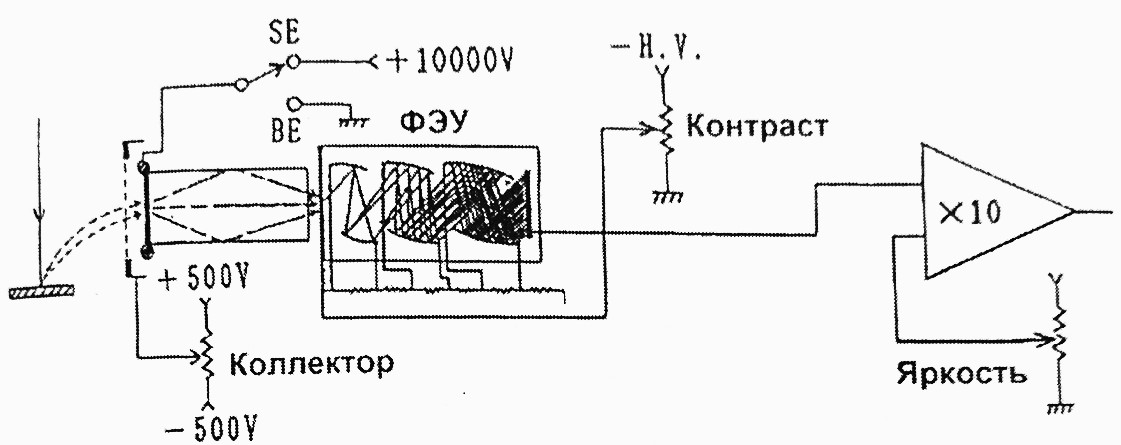
\includegraphics[scale=0.50]{Kollektor_page-0001.jpg}}
        	\caption{Детектор вторичных электронов Эверхарта-Торнли.}
        	\label{детектор ВЭ}
            \end{figure}        

        \subsubsection{Детектор отраженных электронов}
        
\noindent Если вторичные электроны за счёт рассеяния в толще образца вылетают изотропно, то отраженные - направленным пучком в одну сторону. При этом основная масса отраженных электронов направлена навстречу падающему пучку. Они обладают большей энергией, поэтому в РЭМ для их регистрации используется менее чувствительный твёрдотельный детектор. Детектор изготавливается в форме кольца, охватывающего первичный пучок электронов. Кольцо разделено на две половины, каждая из которых функционирует как отдельный детектор. Прецизионный усилитель может измерять либо разностный, либо суммарный сигнал этих двух детекторов, так реализуется возможность получения изображения в элементном или топографическом контрасте.

        \subsubsection{Детектор рентгеновского излучения}
        
\noindent Существует два типа детекторов: волновой и энерго-дисперсионный.

\medskip
            
\noindent Волновой детектор представляет из себя монохроматор, который выделяет из полного потока излучение лишь определенной длины волны. Роль такого монохроматора играют кристаллы-анализаторы. В них, в соответствие с условием Брэга-Вульфа , излучение распределяется по углу в зависимости от длины волны.

\medskip
            
\noindent Энергодисперсионный детектор преобразует энергию каждого фотона излучения в пропорциональный энергии сигнал напряжения. Этот процесс происходит в три стадии. Падающий на полупроводниковый детектор рентген вызывает образование неравновесной электронно-дырочной пары. Затем с помощью предусилителя неравновесный заряд преобразуется в сигнал напряжения. Далее этот сигнал для измерения поступает на вход импульсного процессора.        

    \subsection{Формирование изображения в РЭМ}
	
\noindent Из названия микроскопа ясно, что это растровое устройство, то есть изображение получается не целиком, а формируется поточечно. Облучая тонким электронным пучком одну точку на образце, мы в одном режиме регистрируем истинно вторичные электроны, а в другом – упругоотраженные.

\medskip
        
\noindent Для получения целостной картины поверхность образца сканируется электронным зондом последовательно в каждой точке. Электронный зонд переходит от точки к точке путем отклонения пучка с помощью пары электромагнитных катушек, находящихся перед последней объектной линзой, создающих магнитное поле поперёк зонда, и пучок немного заворачивает вокруг силовых линий. Подавая на электромагниты пилообразное напряжение развёртки, можно водить зондом по поверхности исследуемого образца.

\medskip

\noindent Усиленный сигнал с детекторов электронов задает яркость точки растра получаемого изображения. частота сканирования и число строк могут изменяться в широких пределах. Монитор формирует чёрно-белое изображение, на котором градациями серого цвета соответствуют градации интенсивности потока истинно вторичных или упругоотраженных электронов.

\medskip
        
\noindent Расстояние между строками растра не имеет смысла делать меньше, чем размер исследуемой растровым микроскопом точки. Сканирование в горизонтальном направлении носит не дискретный характер, так как показания детекторов электронов являются непрерывными.

\medskip

\noindent Частота сканирования и число строк могут изменяться в широких пределах, при этом качество изображения характеризуется параметром сигнал/шум, показывающим соотношение интенсивности информационного сигнала в данной точке к шумовому сигналу.
	
\section{Результаты экспериментов}

    \subsection{Особенности изображений биологических объектов}

        \begin{figure}
    	\centering{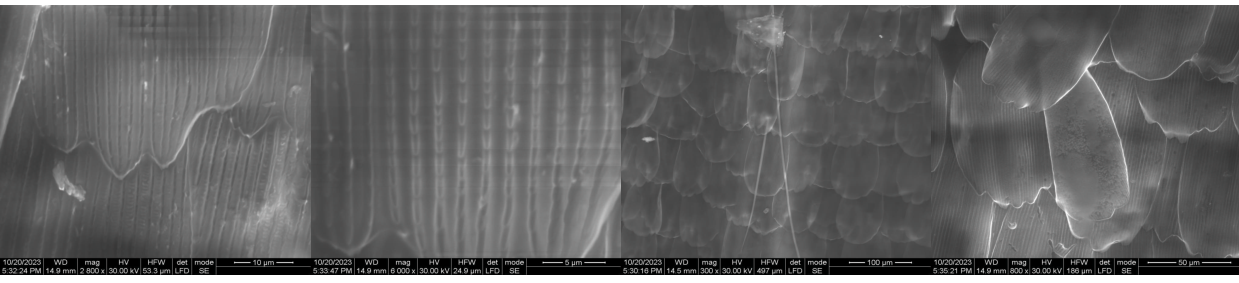
\includegraphics[scale=0.80]{butterfly wing.pdf}}
    	\caption{Изображение крыла бабочки}
    	\label{бабочка}
	\end{figure}

\noindent К сожалению, изображения при проведении работы не были сохранены, поэтому на рис. \ref{бабочка} представлено изображение крыла бабочки в РЭМ в режиме сбора отражённых электронов (BSE-режим), найденное в Интернете. Тем не менее и на этом примере можно выявить характерные черты изображения.

\medskip

\noindent Так, крыло бабочки, оказывается, имеет непростую структуру, а состоит из отдельных чешуек, причём они расположены периодически. Именно этим, кстати говоря, можно объяснить переливание цвета крыльев бабочек: на периодических структурах свет, как изветсно, дифрагирует, и для глаза выделяются те цвета, на длинах волн которых происходит конструктивная интереференция.

\medskip

\noindent Другая интересная характеристика изображения в отражённых электронах -- отсутствие полутонов -- области являются или светлыми, или тёмными, в зависимости от того, попадают ли они падающие в эти области электроных на детектор. Однако на эту картину накладывается также зависимость сигнала от заряда ядер атомов вещества крыла бабочки: чем больше атомный номер, тем сильнее сигнал (т.е. изображение ярче).

\medskip

\noindent Более того, края чешуек сильно контрастны, также как и какие-то "нити"/"усы" на изображении. Дело в том, что с краёв до детектора может добраться гораздо больше электронов. Эта же черта характерна и для объектов, характерный размер которых сравним с глубиной выхода электронов.

    \subsection{Изображения образцов в различных режимах работы РЭМ}

\noindent Контактные материалы на основе CuCr довольно популярны при изготовлении средневольтных вакуумных выключателей. Дело в том, что этот сплав имеет зернистую структуры, что позволяет при необходимости его легко деформировать/раскалывать. Эту зернистую структуру можно пронаблюдать в различных режимах работы РЭМ (см. рис. \ref{CuCr}).

\medskip

        \begin{figure}
    	\centering{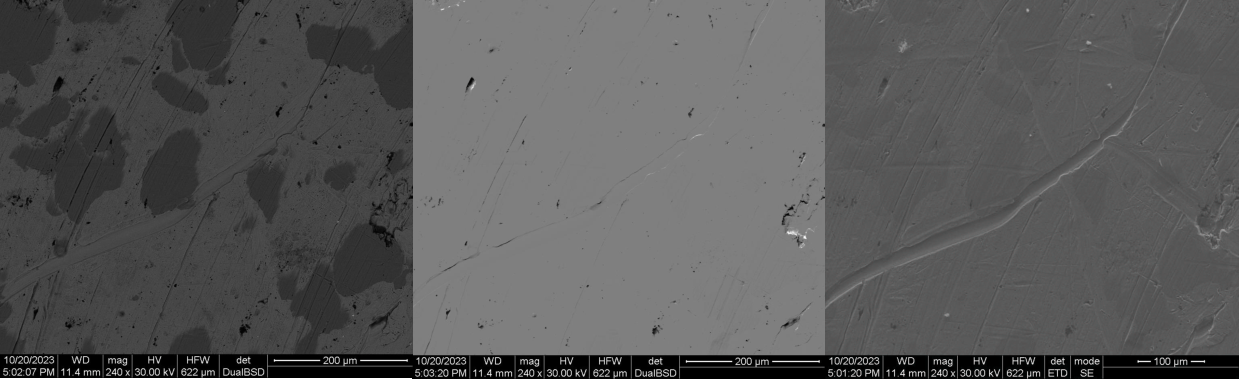
\includegraphics[scale=0.80]{CuCr_SEM_modes.pdf}}
    	\caption{Изображения сплава CuCr в различных режимах работы РЭМ (слева-направо): сбор истинно вторичных электронов; элементный контраст; топографический контраст}
    	\label{CuCr}
	\end{figure}

\noindent Режим медленных, истинно вторичных, электронов используется в РЭМ чаще всего. По отношению к обсуждавшемуся выше изображенияю в отражённых электронах изображение во вторичных электронах содержит полутона, не такое контрастное и имеет больше деталей. Рассматриваемый режим работы обеспечивает на несколько порядков большую глубину фокуса, чем у оптического микроскопа. Прежде всего дело тут в том, что нет жёстких соответствий между плоскостями объекта и изображения: электронные линзы лишь формируют пучок, освещающий образец.

\medskip

\noindent В этом пункте важно отметить, что в режиме отражённых электронов если объект имеет неоднородный состав и нетривиальную геометрию поверхности, то возможно отдельно выделить информацию о составе и о геометрии поверхности. Это связано с работой парного детектора. Наблюдаемые же отличия видны на картинке. Так, зернистая структура не наблюдается в топографическом режиме, ведь она не сильно связана с геометрией поверхности. Аналогично, "царапин" не видно в контрастном режиме, ведь он не чувствителен к геометрии.

    \subsection{Зарядка исследуемого образца при исследовании объектов с использованием РЭМ}
        
\noindent Если электронный пучок облучает заземленный проводящий образец, избыточный заряд просто стекает на землю. Если образец является диэлектриком, заряд может накапливаться на поверхности образца, что в свою очередь портит качество изображения, так как электрическое поле воздействует на эмитируемые вторичные электроны.

\medskip
        
\noindent В нашем наблюдении в процессе сканирования шарика пенопласта, на образце накапливается отрицательный заряд. Мы получили изображение пенопластового шарика (см. рис. \ref{пенопласт}), а после уменьшения ускоряющего напряжения при исследовании того же образца мы получили изображение камеры микроскопа. Во втором случае электроны с меньшей кинетической энергией уже не способны достичь образца из-за электростатических сил взаимодействия, пенопласт отталкивает электроны в разные стороны, они попадают на другие объекты камеры микроскопа, после чего попадают в детектор.

\medskip

\noindent Для снятия заряда в установку производится напуск воздуха. В его составе, например, легко поляризующиеся молекулы воды притягиваются образцу и, зарядившись, уносят заряд. Поэтому рекомендуется проводить исследование диэлектрических образцов в низком вакууме. В работе -- порядка $0.45\cdot10^{-5}$ Торр.

 
    \subsection{Характерные черты изображения внутренней камеры РЭМ}

        \begin{wrapfigure}[14]{r}{0.55\textwidth}
            \centering
            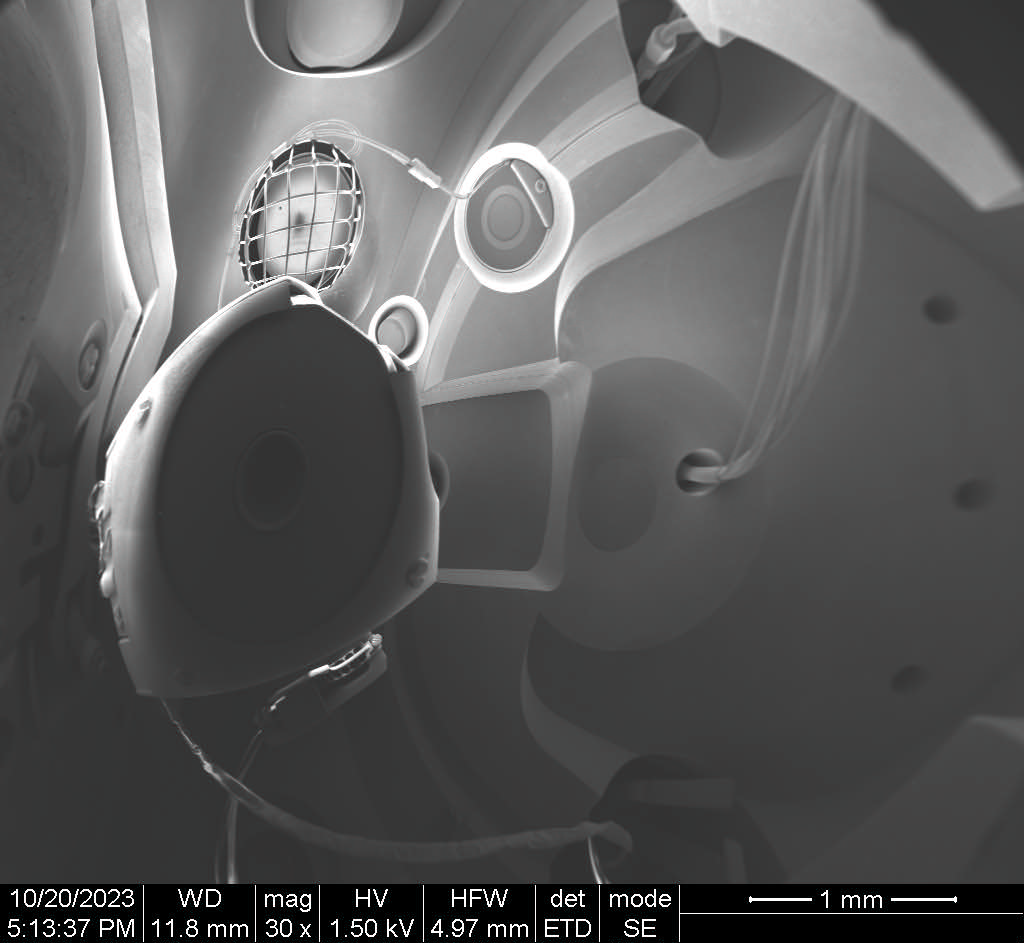
\includegraphics[scale=0.19]{MIRROR.jpg}
        	\caption{Изображение внутренней камеры микроскопа}
        	\label{камера}
        \end{wrapfigure}
 
\noindent На рис. \ref{камера} показано изображение внутренней камеры микроскопа в режиме сбора истинно вторичных электронов. Опять же, чем меньше электронов попадает на детектор, тем слабее сигнал от рассматриваемой области камеры, и она выглядит темнее. Резкие края (например края столика в камере) сильно выделяются, т.к. вероятность попадания электронов с них на детектор более высока.

    \subsection{Определение толщины микроструктуры на чипе}

\noindent К сожалению, изображения при проведении работы не были сохранены. Поэтому ограничимся лишь объяснением вопроса. При повороте камеры меняется угол падения первичного пучка электронов на исследуемую поверхность. Это влечёт изменение изображения, т.к. коэффициент вторичной эмиссии электронов, а также коэффициент отражения зависят от угла падения пучка на поверхность структуры. Если вы посмотрите на свою кисть и будете её поворачивать, вы заметите подобный эффект. Численная его характеристика -- это изменение линейных размеров. Один из таких размеров и предполагалось определить.

\section{Вывод}
	
        В ходе работы были:

        \begin{itemize}
        
            \item изучены физические принципы работы РЭМ и формирования изображений;
            
            \item получены и проанализированы изображения крыла бабочки, сплава CuCr, диэлектрика, камеры микроскопа в различных режимах работы РЭМ.

        \end{itemize}


\end{document} % end of the document
